\section{EMS - ED application}

\subsection{Application}

The system defined in section [ ] 
% TODO: Reference appropriate section
can be directly applied to a healthcare scenario.
The two queueing systems can be thought of as two Emergency Departments (ED) and 
the distributor as the Emergency Medical Services (EMS) that distributes 
individuals to them.
These individuals are patients of the corresponding Emergency Department 
that are sent to.

The parameters of the model described in section [ ]
% TODO: Reference appropriate section
can also be mapped into parameters of the ED and the EMS.

\begin{itemize}
    \item \( \lambda_2 \): The rate of patients that the EMS receives
    \item \( \lambda_{1_i} \): The arrival rate of other patients to ED \(i\)
    \item \( \mu_i \): The service rate of patients the ED \(i\)
    \item \( C_i \): The number of available resources in ED \(i\)  
    \item \( T_i \): The strategy that ED \(i\) chooses to play
    \item \( N_i \): The patient capacity of ED \(i\)
    \item \( M_i \): The parking capacity of ED \(i\)
    \item \( R \): The time target for both EDs
    \item \( \alpha \in [0, 1] \) : \textit{Importance} of blocking time and lost 
    individuals (equation \ref{eq:obj-distributor})
\end{itemize}

The patients that are distributed by the EMS arrive at the hospital via an 
ambulance and are then either unloaded at the ED or remain blocked outside in 
the ambulance.
Whether or not the ambulance and the patient remain blocked is determined by 
the threshold that the given ED chooses to play.
High threshold indicates that the ED accepts patients even if it is relatively 
full, while low threshold means that the ED blocks ambulances more easily.

The game to be played now is between the two EDs and the EMS. 
The strategies of the two EDs are the range of thresholds that they can choose
from and their utilities is the proportion of individuals whose time in the 
system lie within a predetermined target time.
The EMS has to decide how to distribute its patients among the two EDs so that 
the blocking time of ambulances is minimised. 
Note that the formulated game here assumes that prior to making a choice the 
EMS knows the strategies that each ED is playing. 

% TODO: Add a figure to show the applied game

\subsection{Data Analysis}

This subsection aims to analyse how the gaming framework can affect the 
performance measures of the queueing systems and how to escape certain 
inefficient situations.
To study such effects a new concept is introduced that considers the ratio 
between the best possible performance measure and the one that is being
played by the players.
This new concept is defined as the compartmentalised price of anarchy of the 
players of the game and is defined as \(PoA_i(P, s)\), where \(i \in [1, 2]\) 
to distinguish among the two players, \(P\) denotes the performance measure 
function to be used and \(s\) is the strategy that is being played by player 
\( i \). 
The compartmentalised price of anarchy aims to measure inefficiencies in the 
model.
For instance the \(PoA\) for the blocking time of player \(i\) is given by:

\begin{equation}\label{eq:poa_compartmentalised}
    % TODO: Make sure this equation makes sense
    PoA_{i}(B, s) = \frac{B_i(s)}{\min_{\bar{s} \in S_i} B_i(\bar{s})}
\end{equation}

% TODO: Remove \newpage from here
\newpage
Consider a game with the following parameters:

\begin{multicols}{3}
    \begin{itemize}        
        \item \( \lambda_{1_1} \) = 4.5
        \item \( \mu_1 \) = 2
        \item \( C_1 \) = 3
        \item \( T_1 \in [1, N_1] \) 
        \item \( N_1 \) = 6
        \item \( M_1 \) = 5

        \columnbreak
        \item \( \lambda_{1_2} \) = 6
        \item \( \mu_2 \) = 3
        \item \( C_2 \) = 2
        \item \( T_2 \in [1, N_2] \)
        \item \( N_2 \) = 7
        \item \( M_2 \) = 4
        
        \columnbreak
        \item \( \lambda_2 \) = 10.7
        \item \( R \) = 2
        \item \( \alpha \) = 0.9
    \end{itemize}
\end{multicols}

Using equation (\ref{eq:poa_compartmentalised}) and asymmetric replicator 
dynamics (described in section [ ])
% TODO: reference asymmetric replicator dynamics
the game can be simulated and show the compartmentalised price of 
anarchy at every iteration for each ED.
Figure \ref{fig:ard_original} shows the strategies that are being played and 
the values of \(PoA_1(B, s)\) and \(PoA_2(B, s)\) for all iterations of the 
learning algorithm until it reaches an evolutionary stable pair of strategies.

\begin{figure}[H]
    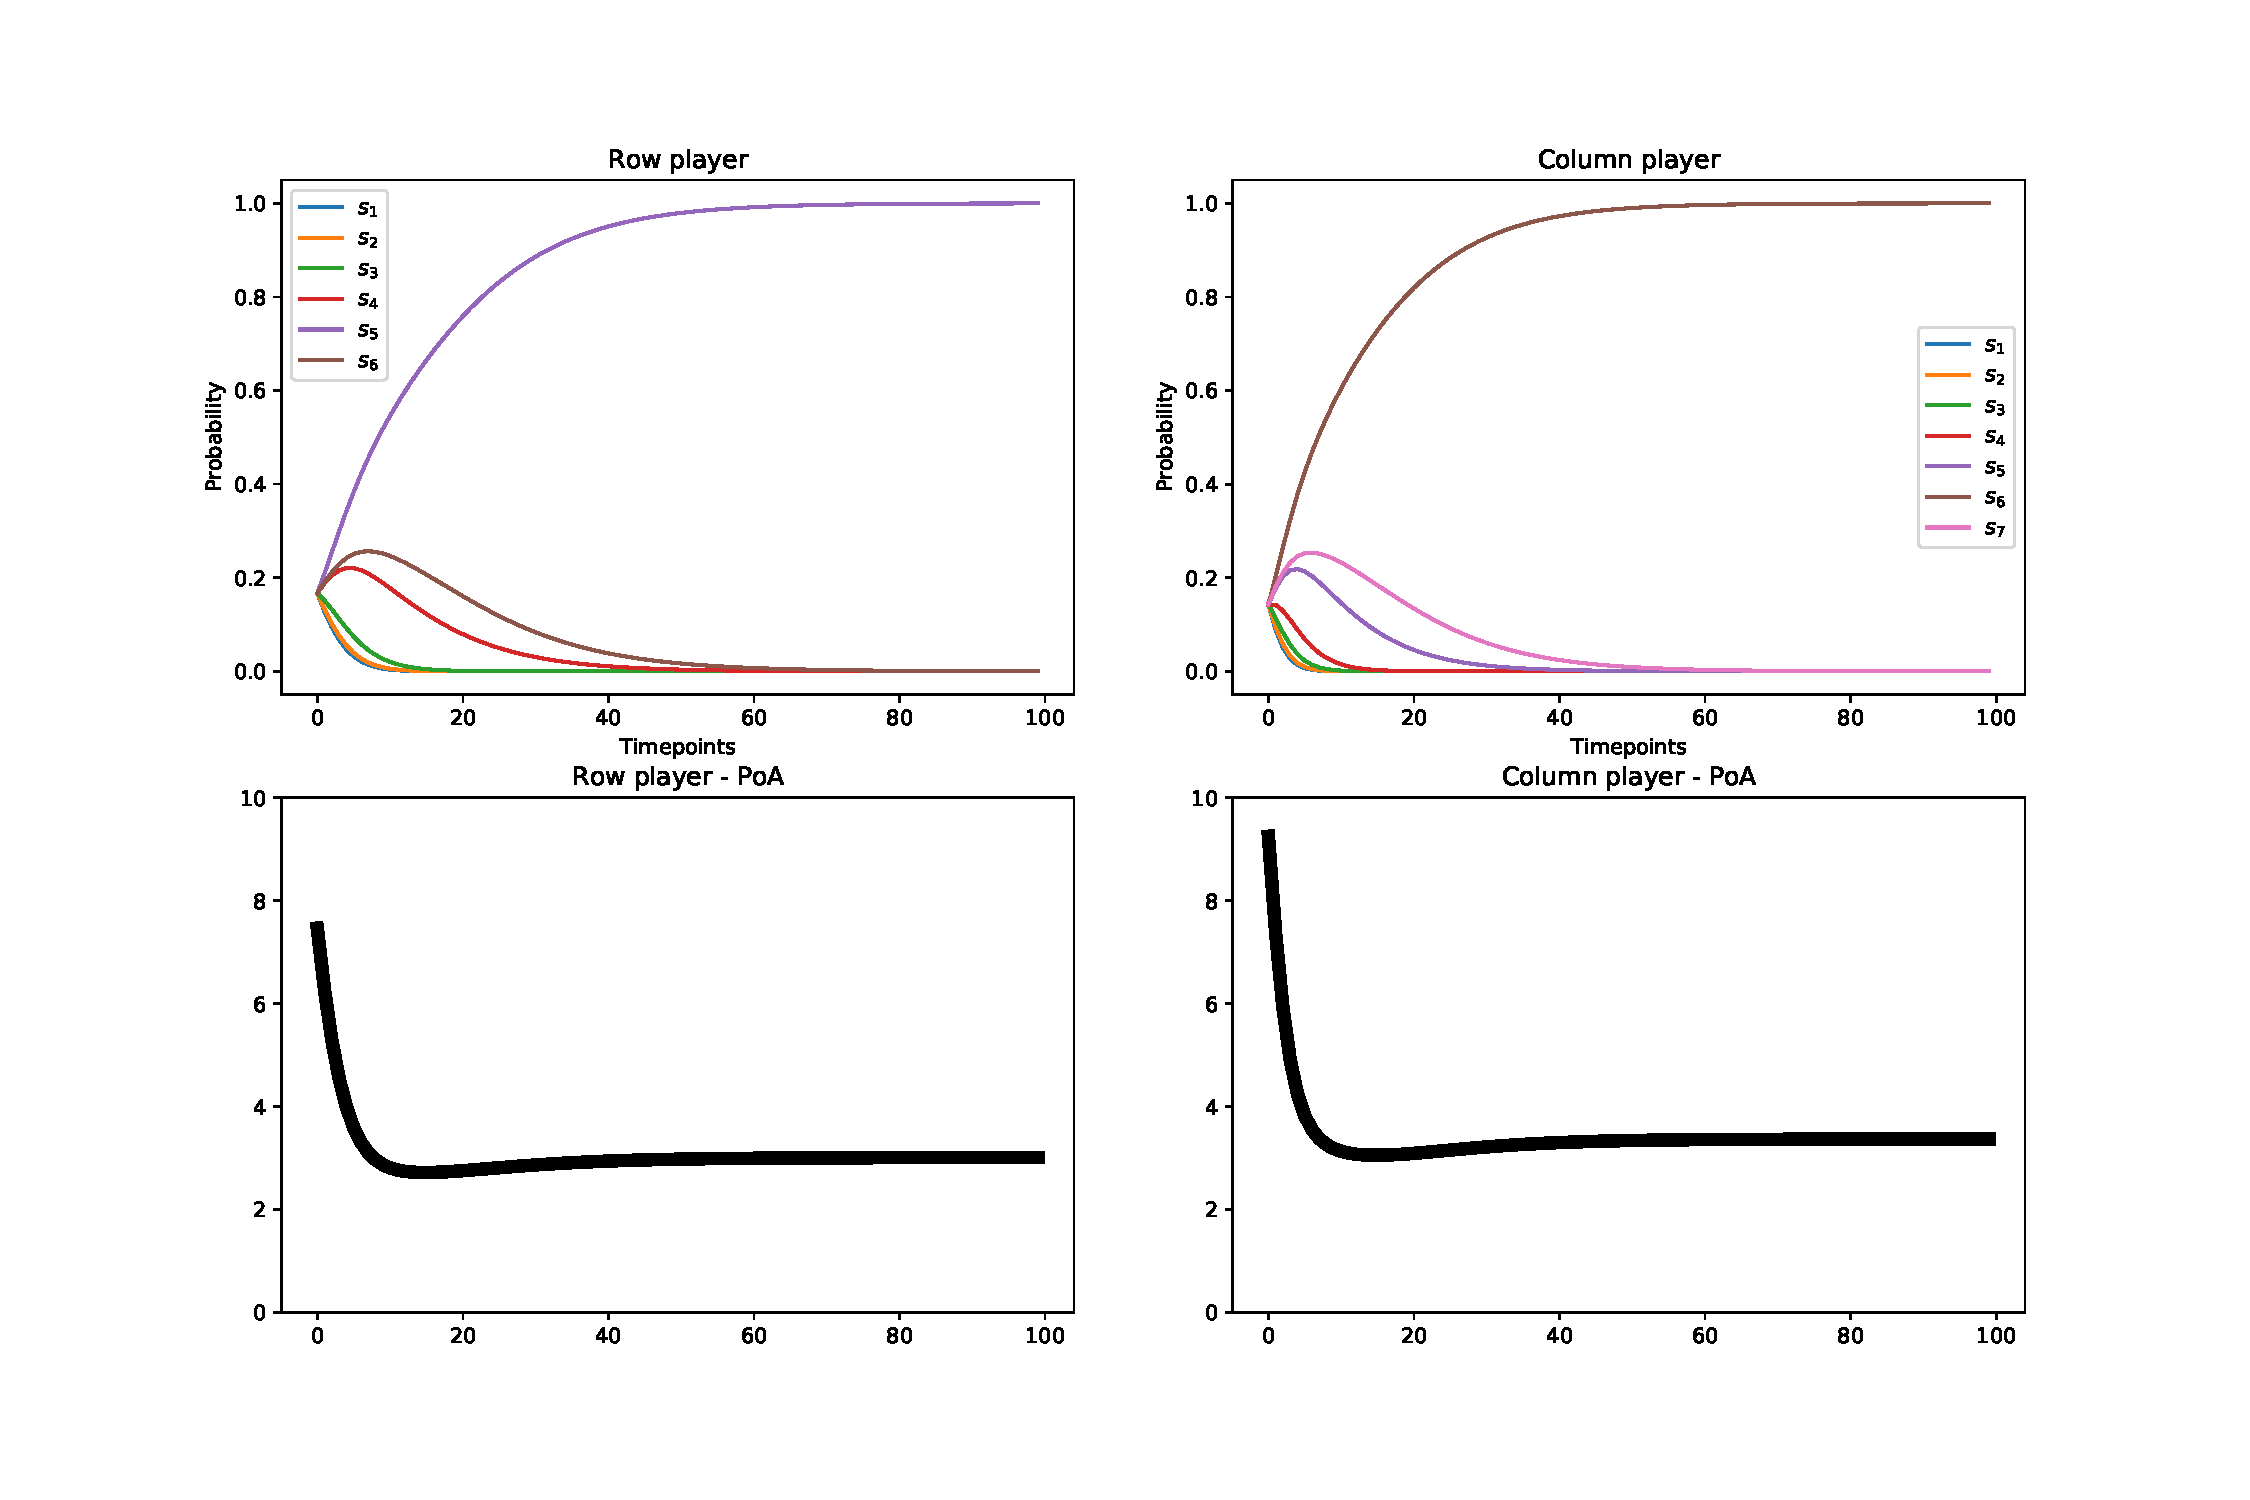
\includegraphics[width=\textwidth, trim=0 400 0 0]{imgs/asymmetric_rd_and_PoA/asymmetric_original.pdf}
    \caption{The strategies played when running asymmetric replicator dynamics
    along with the compartmentalised price of anarchy of the blocking time at
    each iteration of the learning algorithm}
    \label{fig:ard_original}
\end{figure}

It can be observed that the learning algorithm reaches a stable pair of 
strategies where \(T_1 = 5\) and \(T_2 = 6\). After a number of iterations the
price of anarchy for both players stabilises and barely increases until the 
final iteration. 

Figure \ref{fig:ard_lambda_2} shows a similar run of the
algorithm but when the strategies begin to stabilise a huge increase in the
arrival rate of ambulances occurs (i.e \( \lambda_2 = 10.7 \)).


\begin{figure}[H]
    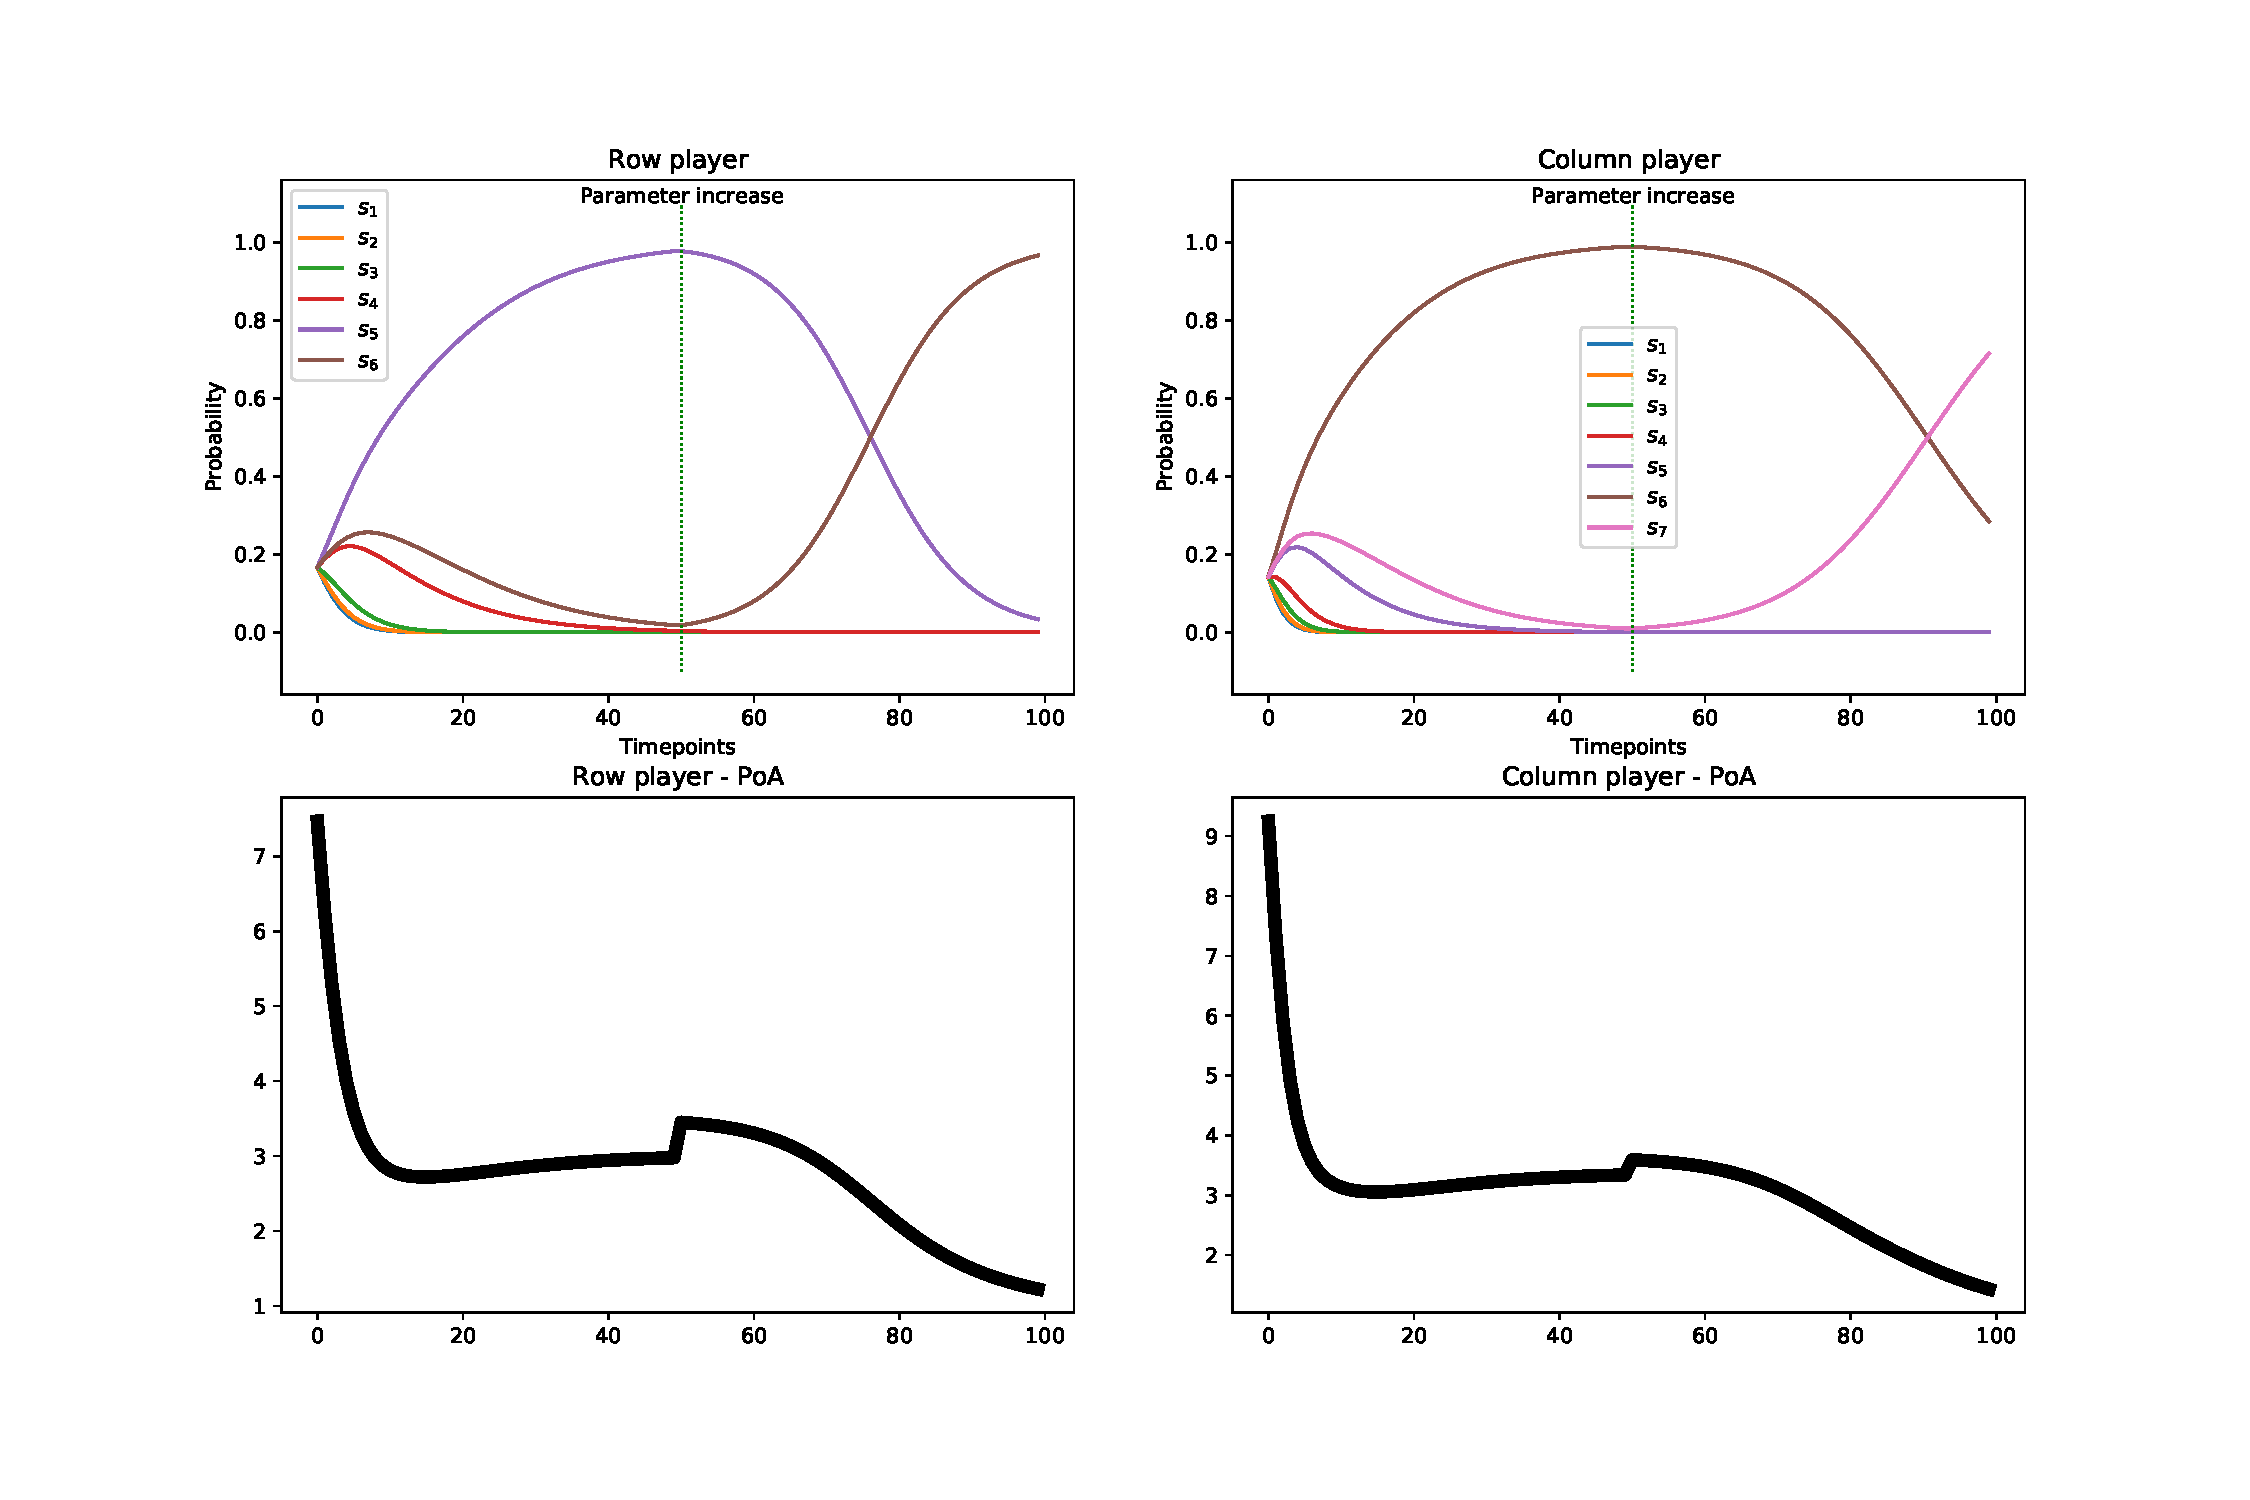
\includegraphics[width=\textwidth, trim=0 400 0 0]{imgs/asymmetric_rd_and_PoA/asymmetric_flooding.pdf}
    \caption{The strategies played when running asymmetric replicator dynamics
    along with the compartmentalised price of anarchy of the blocking time at
    each iteration of the learning algorithm. After a number of iterations the 
    arrival rate of ambulance patients is significantly increased to flood the
    system completely \( \lambda_2 = 10.7 \).}
    \label{fig:ard_lambda_2}
\end{figure}


By increasing \(\lambda_2\) there is no change in the how the players behave
(\(T_1 = 5, T_2 = 6\)), but the outcome of the system does change. 
There is a decline in the price of anarchy of the blocking time which at first 
glance indicates that upon flooding the system it becomes more efficient. 
This is non-sensical though.
What it really shows is that the steep increase in \( \lambda_2 \) simply leaves 
less potential for improvement. 

Figure \ref{fig:ard_num_of_servers} shows a run of asymmetric replicator 
dynamics with a change in the number of servers of both models.
The number of servers are increased from \(C_1 = 3, C_2 = 2\) to 
\(C_1 = 4, C_2 = 3\).


\begin{figure}[H]
    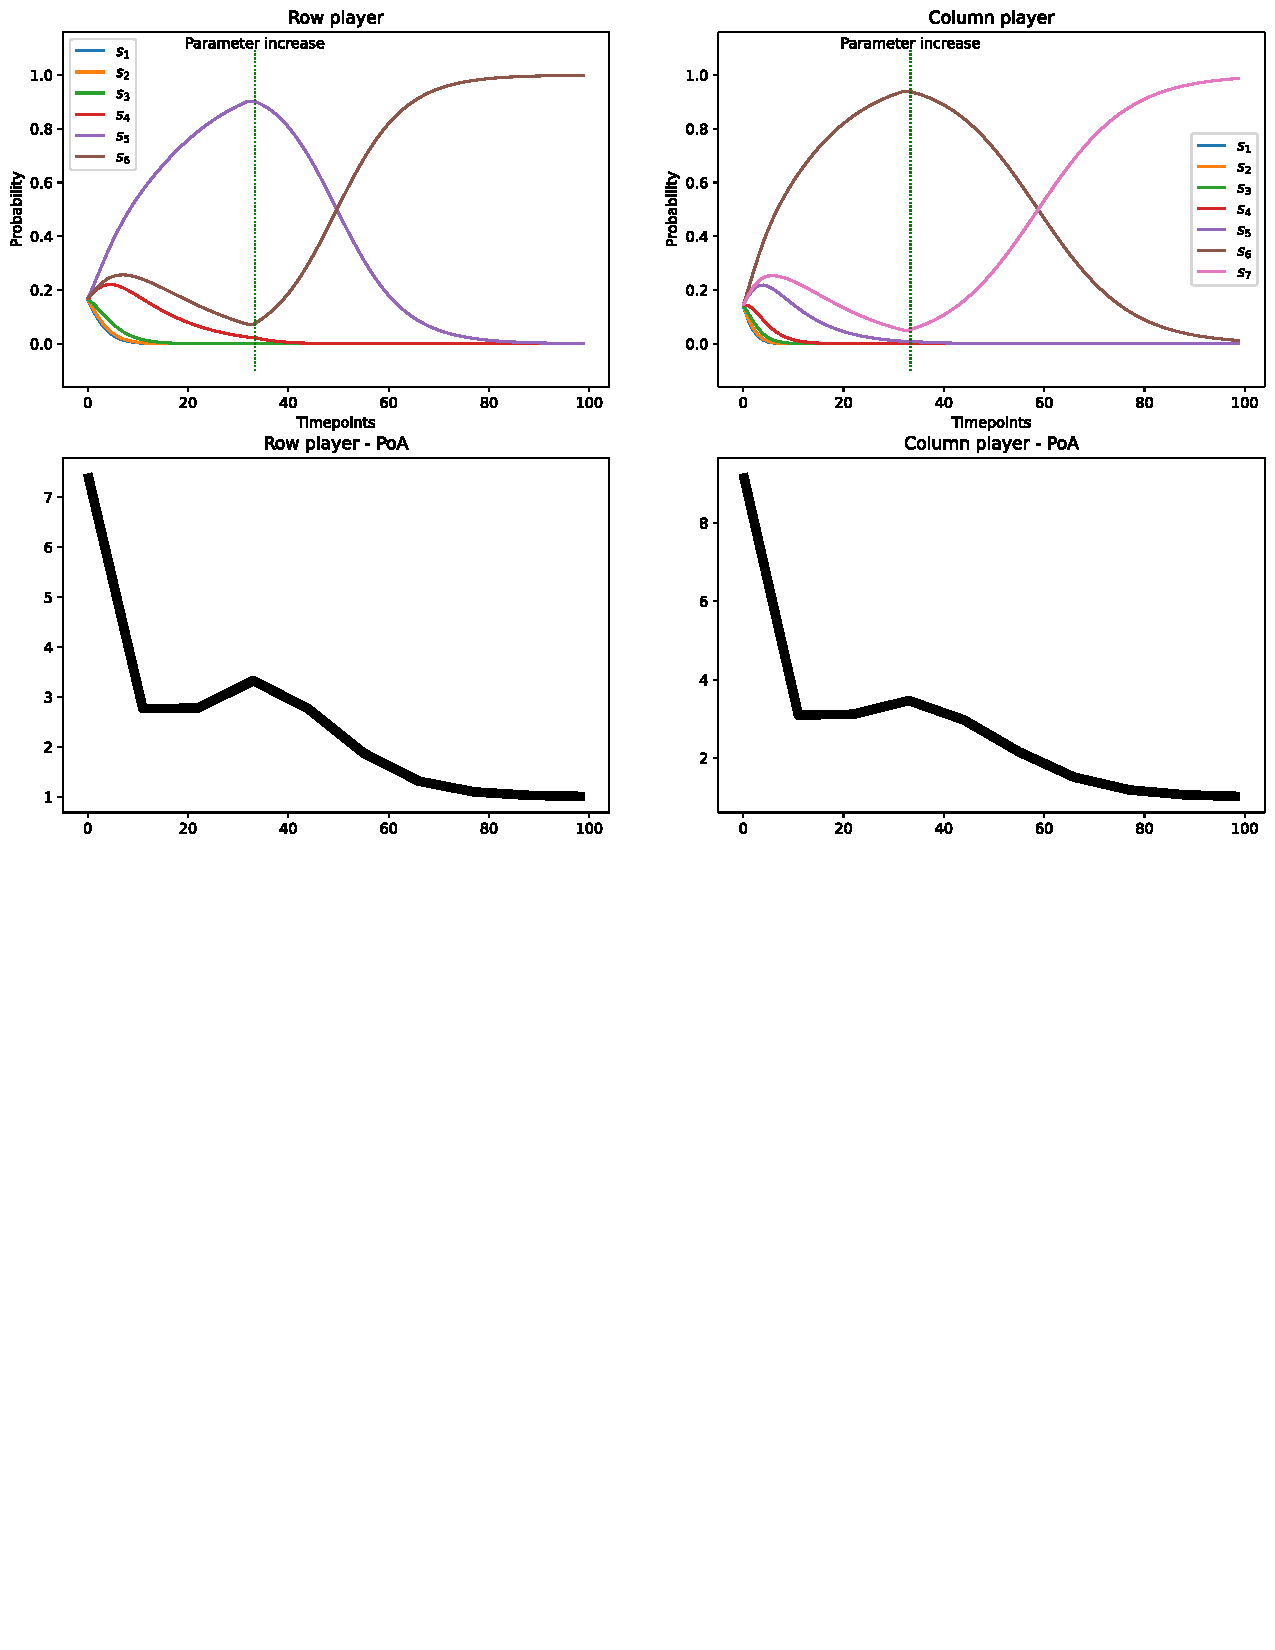
\includegraphics[width=\textwidth, trim=0 400 0 0]{imgs/asymmetric_rd_and_PoA/asymmetric_increase_C.pdf}
    \caption{
        The strategies played when running asymmetric replicator dynamics
        along with the compartmentalised price of anarchy of the blocking time 
        at each iteration of the learning algorithm. After a number of 
        iterations the number of servers for both systems are increased by one.
    }
    \label{fig:ard_num_of_servers}
\end{figure}

In this case the both the behaviour as well as the price of anarchy change.
The players change their strategies from \(T_1 = 5, T_2 = 6\) to 
\(T_1 = 6, T_2 = 7\) and the \(PoA\) of the blocking time goes down.
By adding more resources to the models they are able to increase their 
efficiency.
Although this is a good way to escape such inefficiencies, it might not always
be cost efficient.

Figure \ref{fig:ard_penalty} is slightly different than the previous ones.
Once asymmetric replicator dynamics becomes stable on some inefficient 
strategies (in terms of the blocking time) the payoff matrices of the two are
scaled in such a way so that the selected strategy is penalised.

\begin{figure}[H]
    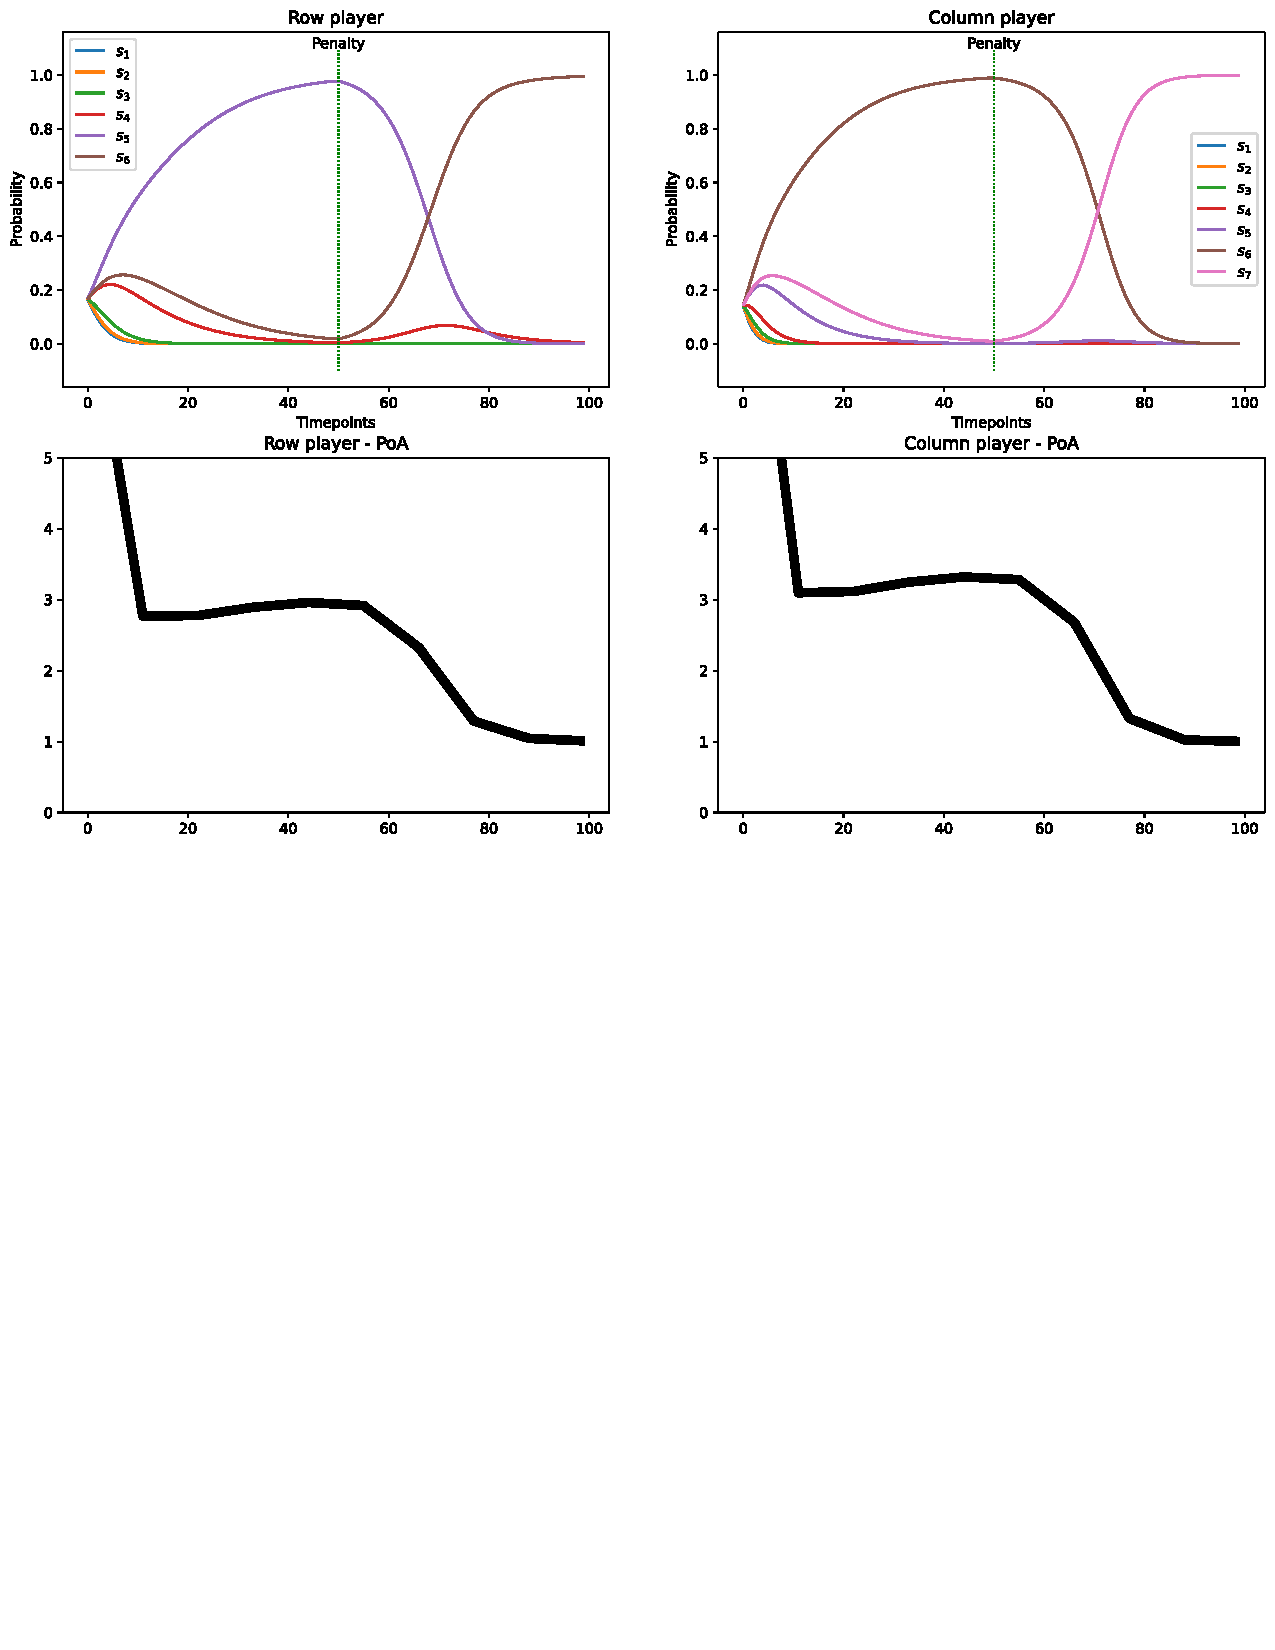
\includegraphics[width=\textwidth, trim=0 400 0 0]{imgs/asymmetric_rd_and_PoA/asymmetric_penalty.pdf}
    \caption{
        The strategies played when running asymmetric replicator dynamics
        along with the compartmentalised price of anarchy of the blocking time 
        at each iteration of the learning algorithm. After a number of 
        iterations the most dominant strategy is being penalised.
    }
    \label{fig:ard_penalty}
\end{figure}

By incentivising the players in such a way the players change their strategies 
and ambulance patients are accepted in the ED more often.
Thus the blocking time \(PoA\) for both EDs drops down. 
